\documentclass[11pt]{article}

\usepackage{geometry}
\geometry{margin=2cm}
\usepackage{graphicx}
\usepackage{hyperref}
\usepackage{amsfonts}
\usepackage{caption}
\usepackage{subcaption}
\usepackage{amsmath}
\usepackage{amsthm}
% for defining definitions
\newtheorem{defn}{Definition}


\hypersetup{colorlinks=true, linkcolor=blue, urlcolor=blue}
\urlstyle{same}
\begin{document}
	
	\author{Aayush Arya}
	\date{(Submitted: \today)}
	\title{}
	
	\maketitle
	
	\hrule
	\begin{center}
		PHY350 WTP-2\\
	 	 \quad Registration No.: 11912610 \quad Section: G2903
	\end{center}
	\hrule
	
	\subsection*{Problem 1}
	The data is plotted below and has a slope of $-5.5$ at $t=20$s.
	\begin{figure}[h!]
		\centering
		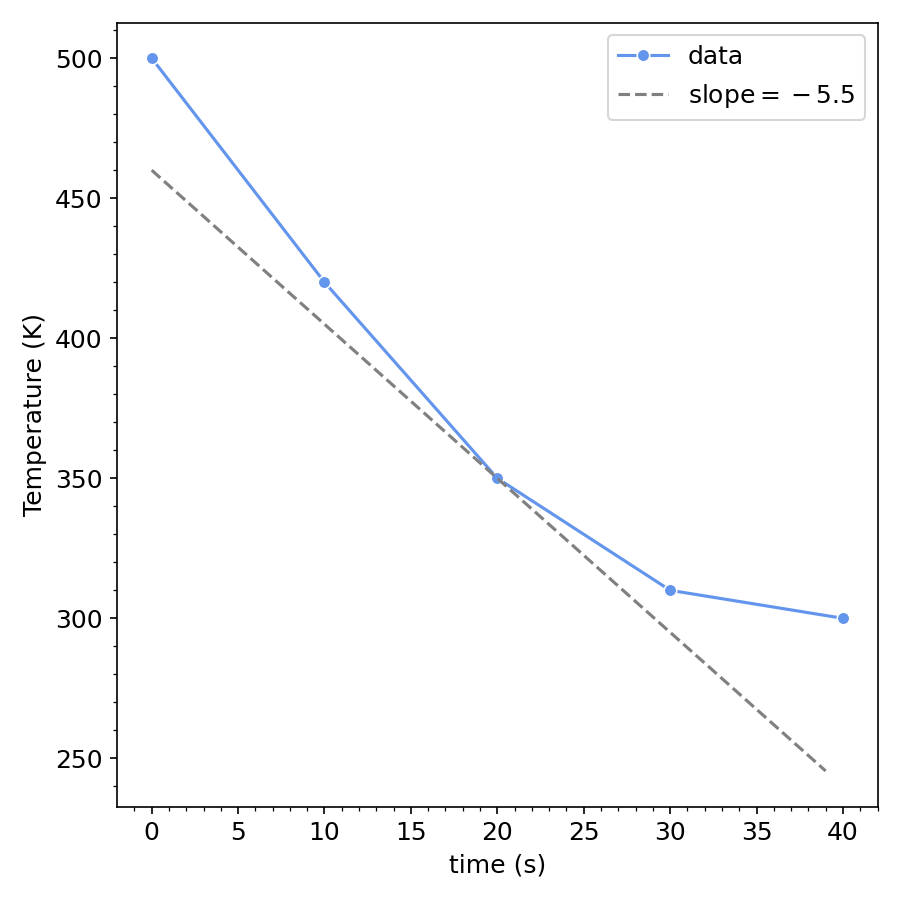
\includegraphics[width=0.6\textwidth]{problem1}
		\caption{The given data has a mean slope of $m=-5.5$ at $t=20$s.}
	\end{figure}

	\subsection*{Problem 2}
	For a charged particle in magnetic field $B$
	\[qvB\sin\theta = mv^2/r \]
		assuming the field is perpendicular
	\[q/m = v/rB\]
	and for an electron with charge $q=-e$,

	\[
	\boxed{
		\frac{e}{m} = -
		\frac{v}{rB}
	}
	\]

	In cases when we know which particle is in the orbit (i.e. $q/m$ is known), the magnetic field $B$ can be estimated from that \[ \boxed{B = \frac{mv}{qr}} \]
	
	
	\subsection*{Problem 3}
	In the leakage method, we have a ballistic galvanometer and a condenser as part of the circuit. A ballistic galvanometer would measure the amount of charge that has discharged through it. 
	
	What we do is, charge a capacitor enough. If we let this charged capacitor flow current through an external circuit by switching on a `key' and then let it discharge. At that point we measure the amount of deflection the galvanometer shows (in degrees, say).
	
	For a large value of $R$, the time constant $RC$ is also sufficiently large and the capacitor discharges slowly. In that case, we can measure the deflection of the galvanometer at later time $t$ to get an estimate of the charged flown until that point. Using the deflections, we get a measure of $Q$ at time $t=0$ and at a later $t=t'$. If the capacitance is known, and we have the deflection and time measurements, we can compute $R$
	
	\[ R = \frac{t}{C\log_e (\theta_0/\theta_t)}\] 
	
	
	\subsection*{Problem 4}
	The B-H and M-H hysteresis loops are related because \[ \vec{B} = \mu_0(\vec{H} + \vec{M})\]
	Since $\vec{H}$ is the applied magnetic field, it's independent of whether the material has saturated (in terms of magnetisation) or not \textemdash it keeps on contributing to increasing $\vec{B}$.
	
	The magnetisation $\vec{M}$ gets saturated and reaches an $\vec{M}_{max}$ for the material in context, giving a zero slope region after that. However, for a B-H loop, the $\vec{B}$ keeps on increasing with increasing $\vec{H}$, with slope $\mu_0$.
	
	\subsection*{Problem 5}
	
	A two probe measurement method (e.g. using a standard multimeter) would add the internal resistivity of the probe device (the multimeter) in the measurement. For precise measurement, however, one would like to avoid this.
	
	In four probe method, the outer two leads provide the test voltage, and the inner two measure the current passing through. Using different leads for the ``test voltage" and the measurement of the current reduce the internal resistivity issue.

	
\end{document}